\documentclass[aspectratio=43]{beamer}
\usetheme{metropolis}

\usepackage{epstopdf,epsfig}

\newcommand{\TITLE}{D-27\\RAW-JENA: Approximate Query Processing for SPARQL Endpoints}
\author{Julien Aimonier-Davat, Minh-Hoang Dang, Pascal Molli, Brice Nédelec, and Hala Skaf-Molli}

\setbeamertemplate{frame numbering}[none]
\setbeamersize{text margin left=0pt,text margin right=0pt}


\usepackage{epstopdf,epsfig}
\usetikzlibrary{arrows.meta}
\tikzset{>={Latex[width=2mm,length=2mm]}}


%%%%%%%%%%% text that goes with the slides %%%%%%%%%%%%%
% We have an awesome query that we want to execute, so naturally we
% execute it on a public SPARQL endpoints, and unfortunately, after 60 seconds
% of execution, i get no results and no insights whatsoever
% on why it failed. I cannot build anything on top of this… sadly…
%
%% So instead, with the same query, we execute it on a same data with
%% our slightly different engine that allows for random walks.  Within a second, I get an
%% online sample and a cardinality estimate of this query, that i can then
%% refine on-demand to get more samples and more accurate estimates.
%%% Such samples represent the cornerstone of many different use
%%% cases, such as join order optimizations, aggregations, processing
%%% summaries of SPARQL endpoints, embeddings, and
%%% exploratory queries.
%%%
%%%% Thank you, feel free to join us on D-27!
%%%% Cheers.


\begin{document}

\newcommand{\X}{10}
\newcommand{\Y}{5}
\newcommand{\FIGUREWIDTH}{0.18\textwidth}
\newcommand{\BOOKMARKCOLOR}{mLightBrown!85}
\newcommand{\BOOKMARKX}{11.5}

\begin{frame}{
    \vspace{-0.5em}
    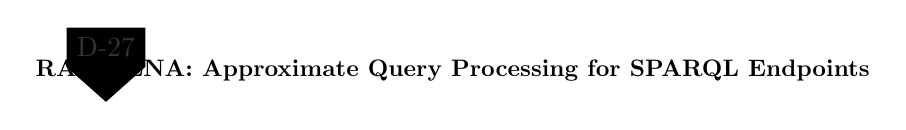
\begin{tikzpicture}
      \node(global_title)[anchor=west, align=left, style={scale=0.86}] at (0,1pt) {\textbf{RAW-JENA: Approximate Query Processing for SPARQL Endpoints}};
      \draw (\BOOKMARKX, 0.33) node(d_27){D-27};
      \filldraw[draw=\BOOKMARKCOLOR, fill=\BOOKMARKCOLOR]
      (d_27.south west) -- (d_27.north west) --
      (d_27.north east) -- (d_27.south east) --
      (\BOOKMARKX, -10pt) -- cycle;
      \draw[color=black!80] (d_27) node{D-27};
    \end{tikzpicture}
  }

  %% begining of the content
  
  \vspace{0.6em}
  \begin{center}
  \begin{tikzpicture}[scale=0.35, every node/.style={scale=0.9}]
    \tiny
    
    %% \draw (0,\Y) node (title_query) {\textbf{An awesome SPARQL query!}};
    %% \draw (title_query.south west) node (request) [anchor=north west,align=left, font=\ttfamily\tiny] {
    %%   SELECT * WHERE \{\\~~~?x1 wdt:P641 wd:Q3609 .\\~~~?x1 wdt:P17 ?x3 .\\~~~?x3 wdt:P361 wd:Q27611 .\\\}};
    
    %% \draw (0,-\Y) node (title_query_bot) {\textbf{An awesome SPARQL query!}};
    %% \draw (title_query_bot.south west) node (request_bot) [anchor=north west,align=left, font=\ttfamily\tiny] {
    %%   SELECT * WHERE \{\\~~~?x1 wdt:P641 wd:Q3609 .\\~~~?x1 wdt:P17 ?x3 .\\~~~?x3 wdt:P361 wd:Q27611 .\\\}};

    %% \draw (0, -0.5*\Y) node (sparql_query) [align=left, font=\ttfamily\tiny, style={scale=0.5}] {
    %%   \textbf{SELECT} ?h1 ?h2 ?h3 ?h4 \textbf{WHERE} \{\\
    %%     ~~?h1 wdd:P31  wde:Q5 .  \# a human being\\
    %%     ~~?h2 wdd:P31  wde:Q5 .  \# another human being\\
    %%     ~~?h1 wdd:P569 ?bd .     \# with a birthdate\\
    %%     ~~?h2 wdd:P569 ?bd .     \# birthdate is identical\\
    %%     ~~?h1 wdd:P570 ?dd .     \# with a date of death\\
    %%     ~~?h2 wdd:P570 ?dd .     \# death date is identical\\
    %%   \}
    %% };

    \draw (0, 0) node (sparql_query) {
      \includegraphics[width=0.27\textwidth]{images/query_example.png}
    };

    \draw (sparql_query.south) node (thinker) [anchor=north east, xshift=-1em, yshift=-1em]{
      \includegraphics[width=0.12\textwidth]{images/democrite.png}
    };

    \draw[color=black!55] (sparql_query.south west) -- (sparql_query.south) -- (thinker.north east) -- (sparql_query.south east);
        

    
    \draw (\X, \Y) node (wikidata) {\includegraphics[width=\FIGUREWIDTH]{logos/wikidata.eps}};
    \draw (wikidata.north) node [anchor=south] (public_endpoint) {\textbf{Public SPARQL Endpoint}};

    \draw (2.5*\X, \Y) node  (sad) {\includegraphics[width=0.21\textwidth]{images/sad.eps}};    
    % \draw (sad.north) node [anchor=south] (timeout) {\textbf{TIME OUT :(}};

    \draw  (\X, -\Y) node [align=center] (raw) {\includegraphics[width=\FIGUREWIDTH]{images/qr-code.png}\\\normalsize \textbf{RAW-JENA}};
    \draw  (raw.south) node [anchor=north](saqp) {\textbf{Approximate Query Processing}};
    

    \draw (2*\X, -\Y) node [align=center] (results) {
      \includegraphics[width=0.3\textwidth]{images/results_example.png}\\\vspace{0.15em}%
      \includegraphics[width=0.3\textwidth]{images/cardinality_example.png}
    };
    \draw (results.south) node[anchor=north] (results_title) {\textbf{Online Sample \& Cardinality Estimates!}};    

    %% \draw  (results.south) node [anchor=north, align=left] (raw_results) {?x1 -> A, ?x3 -> brazil\\?x1 -> B, ?x3 -> equador\\?x1 -> C, ?x3 -> equador\\\\cardinality $\approx 15 \pm 5$};



    \draw (2.9*\X, 0.25*\Y - \Y) node (aggregated_query) {\textbf{\uppercase{Embeddings}}}; %% 4
    \draw (aggregated_query.south west) node [anchor=north west] (join_ordering) {\textbf{\uppercase{Exploratory}}}; %% 5
    \draw (aggregated_query.north west) node [anchor=south west] (embeddings) {\textbf{\uppercase{Summaries}}}; %% 3
    \draw (join_ordering.south west) node [anchor=north west] (summaries) {\textbf{\vphantom{S}\ldots}}; %% 6
    \draw (embeddings.north west) node [anchor=south west] (exploratory) {\textbf{\uppercase{Aggregations}}}; %% 2
    \draw (exploratory.north west) node [anchor=south west] (etc) {\textbf{\uppercase{Join orders}}}; %% 1

    \draw (summaries.south west) node [anchor=north west, xshift=-0.8em] {
      %% from https://pixabay.com/fr/vectors/atlas-monde-mythologie-grecque-7337047/
      \includegraphics[width=0.11\textwidth]{images/atlas.png}
    };

    
    %% \draw[->] (title_query.east) -- (public_endpoint.west);
    %% \draw[->] (title_query_bot.east) -- (saqp.west);
    \draw[->, very thick] (sparql_query.east) -- (wikidata.west);
    \draw[->, very thick] (sparql_query.east) -- (raw.west);

    \draw[->, very thick] (wikidata.east) -- node[anchor=south, font=\small]{>60s\ldots ~ \textcolor{red}{\textbf{TIMEOUT!}}} (sad.west);
    \draw[<->, very thick] (raw.east) -- node[anchor=south]{1s} (results.west);

    \draw [->, very thick] (results.east) -- (aggregated_query.west);
    \draw [->, very thick] (results.east) -- (join_ordering.west);
    \draw [->, very thick] (results.east) -- (embeddings.west);
    \draw [->, very thick] (results.east) -- (summaries.west);
    \draw [->, very thick] (results.east) -- (exploratory.west);
    \draw [->, very thick] (results.east) -- (etc.west);
    
  \end{tikzpicture}
  \end{center}

  \vspace{-0.6em}
  \begin{tikzpicture}
    \draw (0,0) node(univ) {\includegraphics[width=0.1\textwidth]{logos/Logotype_NantesUniversité.eps}};
    \draw (11.4, 0) node(ls2n) {
\includegraphics[width=0.065\textwidth]{logos/LOGOS_LS2N_noir-quadriCMJN.eps}};
  \end{tikzpicture}
  
\end{frame}

\end{document}
